\documentclass{book}
\author{Sam Nolan}
\usepackage{minted}
\usepackage{graphicx}
\usepackage{listings}

\newenvironment{ulist}
	{\begin{itemize}
			\itemsep0em}
	{\end{itemize}}

\newenvironment{xml}
	{\VerbatimEnvironment
	\begin{minted}[tabsize = 2]{xml}}
	{\end{minted}}

\newenvironment{lua}
	{\VerbatimEnvironment
	\begin{minted}[tabsize = 4]{lua}}
	{\end{minted}}
\graphicspath{{images/}}

\newenvironment{yaml}
	{\VerbatimEnvironment
	\begin{minted}[tabsize = 4]{yaml}}
	{\end{minted}}

\newcommand{\hFigure}[2]
	{\begin{figure}[ht!]
		\centering
		\includegraphics[width=90mm]{#1}
		\caption{#2}
	\end{figure}}

\newcommand{\fFigure}[2]
	{\begin{figure}[ht!]
		\centering
		\includegraphics[width=\textwidth]{#1}
		\caption{#2}
	\end{figure}}

\newcommand{\vFigure}[2]
	{\begin{figure}[ht!]
		\centering
		\includegraphics[width=40mm]{#1}
		\caption{#2}
	\end{figure}}

\title{Programming with ProjectX}
\begin{document}
	\pagenumbering{gobble}
	\topskip0pt
	\vspace*{\fill}
	\begin{center}
		\centering
		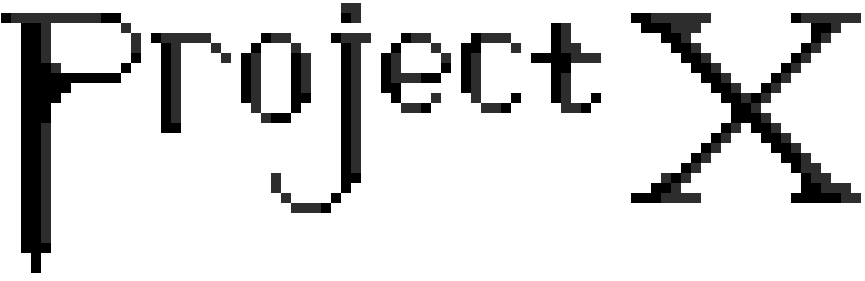
\includegraphics[width=\textwidth]{ProjectX.png}
		Sam Nolan
	\end{center}
	\vspace*{\fill}
	\tableofcontents
	\pagenumbering{arabic}

	\part{Introduction to ProjectX}

	\chapter{Introduction}
	\section{What is ProjectX?}
	ProjectX is both a game and an educational tool for learning the basics of programming. It can be played without even touching the programming aspects as a social multiplayer game, but it becomes much more interesting when players create content of their own through the use of programming languages such as Lua and XML.
	
	ProjectX is a great tool for learning programming for the first time, as it covers a wide range of skill levels. It comes with many tools that help the beginner programmer both get a feel for professional-like environments while being supported along the way. Lua is a great programming language to learn how to code in, because it does not require the programmer to follow strict syntax.
	
	Professionals can also use ProjectX as just a general game. By developing on different parts of the game, every session would be completely different. If teams were to get together to mod this game, or even a classroom, \underline{the changes can be updated into one single game} and can be played multiplayer by everyone. 

	The game is also completely and utterly cross platform. You can run the game on Windows, \underline{Mac}, Linux, Android and \underline{iOS}. Games can also be played \textbf{across platforms}, meaning a person could come along with an Android smartphone, link up to a server hosted by a Linux computer, and play with a tonne of Macintosh and Windows Users!

	\hFigure{CrossPlatform.png}{Cross Platform}

	\section{Game-Play and Rules}
	The game itself is an Role Playing multiplayer game where the objective is to be the last man standing. Players connect to a server, and are spawned into an Arena. The controls are mainly touch based as the game also ports the Android and iOS platforms. Players can roam around a map with the objective of collecting resources to \underline{survive} the harsh environment that they find themselves in. Players will find creatures and other features that can be interacted with. Other players can also be found and they can \underline{choose to team up or to fight,} \underline{last player or team alive wins.}
	
	The game imposes very few constraints about what content can be added to the game. Creature, tiles, interactions, items and much more can be added to the game to make the experience completely different. \underline{Changes that are made to the game} \underline{on one device can be synced} \underline{to another simply by} \underline{on the same game.}
	
	\section{Programming with ProjectX}
	ProjectX has 2 official languages, Lua and XML, as well as YAML in some areas. These languages serve different purposes in the game. XML is used to represent objects in the game, whereas in Lua, actions and procedures can be specified. XML controls map generation, Items, Sprites and many more, whereas Lua controls Creature AI, interactions and Item usage. The skills learnt can be applied to other programming languages such as Javascript, HTML or any other language that a person might want to learn.
	
	Most of the code has its own jurisdiction, as in, the code in each folder will control only a certain aspect of the game, and no more. This is in contrast to most languages, where all code does not need to be in separate files to function. We decided to make ProjectX like this as to keep the code simple as possible.
	
	\section{Installation}
	The installation of ProjectX is reasonably straightforward. Installation is currently supported for linux, Windows and Android. The Android applications have not been released on Google play yet, but are in apk form. In the future, ProjectX should be supported on OSX and iOS. OSX and iOS should theoretically work, but I require a macintosh to develop on those devices.
	
	Because the game is currently in development, receiving a copy of the game can only be done through directly asking Sam Nolan. His contact details can be found in the Acknowledgments.  
	
	Once You have a copy of the installer (ProjectXInstall.exe), the installation is reasonably straightforward. The components that can be installed are explained below
	
	\paragraph{ProjectX}
	ProjectX is the actual game, it is required in the installation.
	
	\paragraph{ProjectX Scripting}
	The official scripting platform for ProjectX, Atom. Comes with auto-complete and error checking for scripting. It is highly recommended if developing with ProjectX.
	
	\paragraph{ProjectX Source Control}
	The Gitkraken source control package. Useful for recording and keeping changes when working in teams, not required.
	
	\paragraph{ProjectX Documentation}
	Contains this book.
	
	\paragraph{ProjectX Sprite Previewer}
	A Sprite Previewer for ProjectX, This application reads a Sprite XML file  and creates sprites to preview before putting in the application. Not required but may be useful for artists.
	
	\section{Acknowledgments}
	This section concerns the developers of ProjectX, contact details are provided for some.
	
	\paragraph{Programming}
	\begin{ulist}
		\item Sam Nolan - NOL0055@bhs.vic.edu.au
		\item Michael Smith
	\end{ulist}
	
	\paragraph{Art}
	\begin{ulist}
		\item Oscar Taylor
		\item Adam Schembri (Codeword Gaming)
		\item Louis Evans
		\item Tom Duchemin
	\end{ulist}
	
	\paragraph{Scripting}
	\begin{ulist}
		\item Hung Dao
	\end{ulist}
	
	\paragraph{Music}
	\begin{ulist}
		\item Louis Evans
	\end{ulist}

	\chapter{Features}
	There are a few feature in ProjectX that should be understood before developing. This chapter is not too important, but does come in handy as a reference for how the game works.
	
	\section{The Arena}
	The Arena is the map and tiles that you can interact with in the game. The arena currently stands at 1500x1500 tiles and takes about 9 minutes to walk across. The map is randomly generated everytime you play the game, and the way it is generated can be coded in XML.

	The Arena refers to each of it's tiles using coordinates, the tile (0, 0) is at the very top of the map, whereas the tile (1499, 1499) is the very bottom, x increases in the right direction, and y increased to the left.

	\subsection{Tile states}
	Every single tile can have a state associated with it, a state is actually a number, but it is used to find out what has happened to the tile and some of it's properties. So far, there are 3 official states, those states are untouched (0), Destroyed (1), Depleted(2). Any tile with a state of 1 (destoyed) will not be shown on the map.
	
	You can invent your own states and use the however you wish, for example, you may have 4: haunted, which means that a ghost will spawn if the player tries to break it.

	\subsection{Tile properties}
	You can associate a table of properties with every tile, this is VERY useful. For example, you might have an apple tree with only a certain amount of apples on it, so you store the amount of apples it has left inside the properties table. Then the player cannot pick apples if there are none left. 
	
	In the same way, you could keep other values in the properties table, for example, the tree might need to be hit a few times with the axe, so it could store how weak it is and fall down when the player has had a certain amount of swings at it.
	
	\subsection{Regions}
	Regions are collections of tiles that are usually geographically close. These can be used to make different biomes, differentiate between areas in lua code and to play music in different regions. For example, in the "standard" map, there is a beach, cliff and snow biome. 
	
	\section{Creatures}
	Creatures can be spawned into the game, and AIs can be made for each creature, all creature AIs are coded in Lua and animations can be made for the creature's movement.
	
	Creatures can represent any entity that is not the player, despite the name, a creature can be also be an NPC along with monsters and other things.
	
	Similar to tiles, creatures can also have a properties table associated with them, creatures have a powerful state-based ai system that can be customized to do a lot of different things.

	Creatures can also have tags associated with them to categorize them. These can be used for any purpose.
	
	\section{Items}
	Items can be given to players, used and crafted. Items are made using the Items XML file.
	
	Inside the Items XML crafting recipes along with item descriptions can be given, multiple crafting recipes can be given to each item.
	
	Items can also execute Lua code with in-inventory uses, these appear as buttons inside the inventory. What happens can be coded using Lua so it again makes items infinitely customizable.
	
	\section{Players}
	You can create players that can be played inside the game.
	
	\part{Developing with ProjectX}
	
	\chapter{Getting started with Developing}
	This section addresses the structure of ProjectX and how to use some of the tools that come with it.
	
	\section{Structure of ProjectX}
	All the ProjectX source files can be found in Local AppData for Windows, that is, \texttt{C:\textbackslash Users\textbackslash [Username]\textbackslash AppData\textbackslash Local\textbackslash ProjectX} The AppData folder is hidden, so you may need to enable seeing hidden files.
	
	This folder can also be accessed by opening it with Atom. The ProjectX Scripting link will automatically direct to the resources folder.
	
	For linux, you will need to build ProjectX from source, just clone the official repository, use cmake and make to build the Project. Boost is required.

	\subsubsection{Log file}
	In the installation directory, there is a "log" folder, which contains a file named \texttt{current.log}. If anything goes wrong while programming, the first thing you should do is check the log file as it may contain useful information as to how to fix your issue. Any lua and xml errors are logged into this file, along with other helpful information. It is possible to log to this file while debugging to help pinpoint where your code goes wrong.

	\subsubsection{Save file}
	Inside the save directory, there is a file named \texttt{SaveFile.yml}. This contains information that has been saved from the game for later usage, using this file, you can also enable a few hidden features. Here is an example of the save file:
	
	In linux, the save file is located at \texttt{~/.config/ProjectX/SaveFile.yml}


	\begin{yaml}	
playerName: Sam Nolan
fullScreen: false
skipSplashes: true
	\end{yaml}

	This file is easy to edit, simply change the values after the colons. Make sure that there is a space after the colon and no space after the propertyName, as shown above.

	You can enable fullscreen by setting \texttt{fullScreen} to \texttt{true} instead of \texttt{false}. The \texttt{skipSplashes} property is not shown by default. If set to true, then the 2 splashes at the start of the game will not show and it will take you directly to the menu page.

	There is also another hidden property, this property is called \texttt{devMode} and if set to true, it will enable the Lua Terminal in game by pressing T.
	\section{Atom}
	Atom is the official scripting platform for ProjectX. The actual Atom project can be found at \texttt{atom.io}. There is a package (or extension) to Atom which contains error checking and code-completion for ProjectX. The package is installed with Atom from the installer.
	
	\fFigure{Atom.png}{Screenshot of Atom}

	Atom contains a file viewer on the left, you can browse through the entire resources directory and look view images and various other things. Atom is used by many proffesional programmers.

	\section{Lua Terminal}
	The Lua terminal can execute lua commands in game and is very helpful starting point for programming in Lua. It is similar to the minecraft terminal except that it will only accept commands and the commands are in lua. The Terminal can be opened with T and will only be available if you enable \texttt{devMode} inside \texttt{SaveFile.yml} (see Save file above). Escape will close the terminal.

	You can execute commands from here (such as \texttt{print("Hello world")}) and the output (if there is any) will show above where you typed it. It will also show any lua errors that happened in the game, so you do not have to check your log file for errors, you can just press T to view it. the \texttt{clear()} function will clear the terminal if it gets clogged up.
	
	You can also view and run previous commands by using the up and down arrow keys. If you wish to perform a multi-line command, you can end the command with the backslash character. This will wait until you input a command that does not end in a backslash to execute the multi-line command.
	
	Another very useful function is the \texttt{help} function, which prints help information about any other function. For example \texttt{help(print)} will return information about the print function, or \texttt{help(player.getPosition)} returns help information about the getPosition function of the player object.

	\chapter{ProjectX XML}
	\section{Beginning With XML}
	XML is called a \textbf{markup language}. A markup language is used to represent objects. It has a certain syntax that uses angle brackets and tags and is nearly identical to HTML in syntax. This is an example of a tag:
	
	\begin{xml}
<class>
	\end{xml}
	
	What makes it a tag is the angle brackets around it, "class" is the \textbf{name} of the tag. In ProjectX there are many different tags that are differentiated by name that have a variety of uses. For example the \texttt{<class>} tag is used in the players XML file to specify a character class.
	
	Every tag has a matching ending tag. The ending tag is the same as the original (starting) tag except that it starts with a forward slash (/)

	\begin{xml}
</class>
	\end{xml}
	
	Anything between the ending tag and the original starting tag is said to be inside the tag, for example:
	\begin{xml}
<description>
	This is a description!
</description>
	\end{xml}
	The "This is a description!" is said to be inside the tag or the description tag's \textbf{value}. We can have tags inside tags like so:
	\begin{xml}
<class>
	<description>
		This is a description!
	</description>
</class>
	\end{xml}
	The description is inside the class and the text is inside the description. You can make many different structures using XML.
	
	In XML, any tag can have \textbf{attributes} associated with it. An attribute looks like this:
	\begin{xml}
<class name="Rat Man">
	
</class>
	\end{xml}
	In this case, \texttt{name} is an attribute of the \texttt{class} tag. and the \textbf{value} of the name attribute is \texttt{"Rat Man"}. In ProjectX, all attribute values are surrounded by quotes. The quotes are not part of the value, but just group the text in between them together. This is called a \textbf{string} and comes in various programming languages. For example, the string \texttt{"Hello World!"} represents the literal value of \texttt{Hello World!}.
	
	That concludes the basics of XML. The following sections show how XML can be used in different areas of the game. It is in order of the easiest things to learn to the hardest.
	
	\section{Sprites}
	The sprites XML file is not necessarily the easiest to learn but is required by the other scripts.

	The sprites XML file contains all the different sprites that will be used in various other aspects of the game, those aspects being players, tiles, creatures and items. Here is an example of a sprites XML file.

\begin{xml}
<items>
	<spritesheet source = "Resources.png" >
		<sprite name="Gold" x="0" y="0" />
		<sprite name="Wood" x="1" y="0" />
		<sprite name="Stone" x="2" y="0" />
		<sprite name="Apple" x="3" y="0" />
	</spritesheet>

	<spritesheet source="StandardTools.png" >
		<sprite name="Pickaxe" x="0" y="0" />
		<sprite name="Shovel" x="1" y="0" />
		<sprite name="Sword" x="0" y="1" />
		<sprite name="Axe" x="1" y="1" />
	</spritesheet>

</items>

<tiles>
	<spritesheet source = "terrain.png" tileWidth = "1" tileHeight = "1" >
		<sprite name="water" x ="0" y="0" />
		<sprite name="sand" x="1" y="0" />
		<sprite name="grass" x="2" y="0" />
		<sprite name="cliff" x ="0" y ="1" />
		<sprite name="stoneFloor" x ="3" y="0" />
		<sprite name="snow" x = "1" y="1" />
		<sprite name="graveStoneFloor" x="2" y="1" />
		<sprite name="graveGrass" x="3" y="1" />
	</spritesheet>

	<spritesheet source = "tree.png" tileWidth = "1" tileHeight = "3" >
		<sprite name="tree" x="0" y = "0" />
	</spritesheet>

	<spritesheet source = "misc.png" tileWidth = "1" tileHeight = "1" >
		<sprite name="coal" x="0" y = "1" />
		<sprite name="mudrock" x = "1"  y="1" />
		<sprite name="coal2" x = "0" y = "0" />
		<sprite name="gold" x = "1" y = "0" />
	</spritesheet>

	<spritesheet source="Small Trees.png" tileWidth = "1" tileHeight = "2" >
		<sprite name="palm" x="0" y="0" />
		<sprite name="shrubbery" x="0" y="1" />
		<sprite name="appleTree" x="1" y="1" />
	</spritesheet>
	<spritesheet source="Supertall Tree.png" tileWidth = "1" tileHeight ="4" >
		<sprite name="SuperTreh" x="0" y="0" />
	</spritesheet>
</tiles>

<creatures>
	<spritesheet source= "Rat anim.png" height= "10" width="16">
		<animate name="Rat Left" height="6" width= "1" x="0" y="0" speed="0.1" />
		<animate name="Rat Right" height="6" width= "1" x="1" y="0" speed="0.1" />
		<sprite name="Rat Left Idle" x="0" y="0" />
		<sprite name="Rat Right Idle" x="1" y="0" />
	</spritesheet>

	<spritesheet source= "BigRatAnim.png" height="13" width="17">
		<animate name="Big Rat Left" height="6" width="1" x="0" y="0" speed="0.1" />
		<animate name="Big Rat Right" height="6" width="1" x="1" y="0" speed="0.1" />
		<sprite name="Big Rat Left Idle" x="0" y="6" />
		<sprite name="Big Rat Right Idle" x="1" y="6" />
	</spritesheet>
</creatures>

<players>
	<spritesheet source="Birdfoot.png" height="30" width="15">
		<sprite name="Birdfoot" x="0" y="0" />
	</spritesheet>

	<spritesheet source = "BigRatAnim.png" height="13" width="17">
		<animate name="Rat Man Left" height="6" width="1" x="0" y="0" speed="0.1" />
		<animate name="Rat Man Right" height="6" width="1" x="1" y="0" speed="0.1" />
		<sprite name="Rat Man Left Idle" x="0" y="6" />
		<sprite name="Rat Man Right Idle" x="1" y="6" />
	</spritesheet>
</players>
\end{xml}
	As you can see, the sprites XML file is split up into sections, those sections being \texttt{<creatures> <players> <tiles>} and \texttt{<items>}. This section seperate the different places where the sprites will be used in the game.

Inside each of these sections are spritesheets, these spritesheets correspond to different files inside the res/sprites folder. Here is a listing of the res/sprites:

\begin{lstlisting}
res/sprites
├── creatures
│   ├── BigRatAnim.png
│   ├── Rat anim.png
├── items
│   ├── Resources.png
│   ├── UltaniumGodbladeAni.png
│   ├── Ultanium.png
├── players
│   ├── BigRatAnim.png
│   ├── Birdfoot.png
│   └── Hot Dog Man.png
└── tiles
    ├── deadlands.png
    ├── Eggstoudanry_Statue.png
    ├── graveMisc.png
    ├── misc.png
    ├── Small Trees.png
    ├── Supertall Tree.png
    ├── terrain.png
    └── tree.png
\end{lstlisting}

The source attribute of the spritesheet tag tells the game where to find the image file. As the folder structure suggests, the sections are split up into their own folders, for organization. Other than the source attribute, the attributes for the spritesheet tag are different for all the different sections, this is because the size of some sprites can be inferred from their context. Items will always be 32x32, while tiles will be in lots of 32 and 24 (width and height respectively). 

Because of this, spritesheets have different attributes for width and height depending on their section, the attributes are as follows:

\paragraph{items} No extra attributes needed, sprites are assumed to be 32x32.
\paragraph{tiles} \texttt{tileWidth} and \texttt{tileHeight} are measured in tiles and outline the tiles size, for width, it is in lots of 32 pixels, for height, it is in lots of 24 pixels
\paragraph{creatures and players} \texttt{height} and \texttt{width} attributes are measured in pixels.

The spritesheet contains many sprites within it, each sprite must be the same size inside the spritesheet. The sprites inside the spritesheet can be specified with the \texttt{sprite} or \texttt{animate} tag. The different between the two is that a sprite is a static image whereas the animate moves and flicks through frames and creates an animation. It is highly recommended that you make animations for players and creatures, tiles and items are acceptable to not be animated.

The sprite tag has a \texttt{name, x} and \texttt{y} attribute. The name is the name of the sprite inside the spritesheet for use later. With items and tiles, this name must correspond with the exact name of the item/tile in the their respective XML files. With creatures and players, it is possible (and recommended) to have multiple sprites associated with on entity. For example there may be a sprite of the creature going right and another of the creature going left. This means that the name of the sprite does not need to match the name of the creature of player, but it should resemble it in some way for clarity.

The \texttt{x} and \texttt{y} attributes specify where the sprite is found on the tilesheet. They start in the top left and move down to the bottom right. For example, consider the image below:


This image contains various floor types, the corresponding spritesheet tag for this spritesheet is as follows:

\hFigure{terrain.png}{Terrain Spritesheet}

\begin{xml}
<spritesheet source = "terrain.png" tileWidth= "1" tileHeight = "1" >
	<sprite name="water" x ="0" y="0" />
	<sprite name="sand" x="1" y="0" />
	<sprite name="grass" x="2" y="0" />
	<sprite name="cliff" x ="0" y ="1" />
	<sprite name="stoneFloor" x ="3" y="0" />
	<sprite name="snow" x = "1" y="1" />
	<sprite name="graveStoneFloor" x="2" y="1" />
	<sprite name="graveGrass" x="3" y="1" />
</spritesheet>
\end{xml}

The animate tag has a few more attributes, to illustrate, We will use the example of the Big Rat. This is the xml for the sprite:
\begin{xml}
<spritesheet source= "BigRatAnim.png" height="13" width="17">
	<animate name="Big Rat Left" height="6" width="1" x="0" y="0" speed="0.1" />
	<animate name="Big Rat Right" height="6" width="1" x="1" y="0" speed="0.1" />
	<sprite name="Big Rat Left Idle" x="0" y="6" />
	<sprite name="Big Rat Right Idle" x="1" y="6" />
</spritesheet>
\end{xml}

\vFigure{BigRatAnim.png}{Big Rat animation}

That attributes for the animate tag are a bit more complicated. the x and y attributes are which sprite the animation starts on, the height attribute is how vertically sized the attribute is. In this case the animation is 6 high because there are 6 sprites that are above each other which will be cycled through. The width is similar. Currently, the animation will run in a top-down left to right order. The speed is how many seconds each sprite should be displayed, in this instance, a sprite is only shown for a tenth of a second.

With this example, there are also normal sprites inside the spritesheet, it is possible to mix animates and sprites in the same spritesheet, it is also possible to have animates and sprites sharing sprites, like the (small) rat example above.

Even though there are no animations for tiles currently, it is entirely possible to do so.

\section{Music}
The support for the music in XML is trivial, and it may be removed in the future as it can be done through Lua. But nevertheless, the music XML file is one of the simplest XML files to learn, here is an example of the music xml file:
\begin{xml}
<region name="plains">
	<song source="Ambient Hope" />
</region>
<region name="snow">
	<song source="Chase in the cold" />
</region>
<region name="beach">
	<song source="Seaside" />
</region>
<region name="graves">
    <song source="Ambient Despair" />
</region>
<region name="cliffs">
	<song source="Grind" />
</region>
<region name="desert">
	<song source="A little warm" />
</region>
\end{xml}

If you think that you understand how this works, you probably do. The region tag is a region of tiles as specified in the map generation XML file. The \texttt{name} attribute is the name of the region. The song tag is the song to be played in that region, and the source is the name of the song to be played. The music can be found in res/music. The current listing of this file is as below:

\begin{lstlisting}
res/music
├── A chase!.wav
├── A little warm.wav
├── Ambient Despair.wav
├── Ambient Hope.wav
├── Ambient Nostalgia.wav
├── Chase in the cold.wav
├── Endgame.wav
├── Grind.wav
├── In the grime.wav
├── My Song 4.wav
├── Rust.wav
├── The Vain King.wav
└── Transformation.wav
0 directories, 13 files
\end{lstlisting}

As you can see, you do not need to include the file extension with the source name. Also, there are many tracks that have not been added to the game yet.

The music XML file may be improved on in the future.

\section{Items}
The Items XML file contains all the things that can be picked up and placed inside your inventory, here is a sample of the Items XML file:

\begin{xml}
<item name="Pickaxe">
	<ingredients>
	Wood:3;
	Stone:3;
	</ingredients>
	<description>
	Tired of smashing a rock with wood?
Now you can do the same... with stone!
	</description>
</item>

<item name="Shovel">
	<ingredients>
	Wood:3;
	Stone:1;
	</ingredients>
	<description>
	For when your hands just aren't enough.
	</description>
</item>

<item name="Axe">
	<ingredients>
	Wood:3;
	Stone:2;
	</ingredients>
	<description>
	Got wood? Now you do! 
Well... soon, at least.
	</description>
</item>

<item name="Sword">
	<ingredients>
	Wood:1;
	Stone:3;
	</ingredients>
	<description>
	For killing the good... and the bad...
and the mediocre.
	</description>
</item>
\end{xml}

These are the basic tools found in ProjectX, the Pickaxe, Shovel, Axe and Sword. The name attribute is the display name of the item and also the exact name of the sprite that will be displayed with the item.

The item tag can have 2 children, the first is the ingredients tag, the tag includes what is needed to craft the item. The ingredients tag is not necessary and the item can be obtained through other ways (like getting it through a lua script). The syntax for the ingredients is simple:

\begin{center}
		\texttt{[item] : [quantity] ;}
\end{center}

Make sure to include the semicolon at the end of the ingredient, it separates them. For example, the statement \texttt{Wood:3;Stone:1;} is perfectly legal, but is not recommended for legibility reasons.

It is possible to have multiple recipes for items, meaning that the item will become craftable when any of the recipes are fulfilled.

The other tag inside the item tag is the description, this is text that is shown with the item, there is a theme of satire with these descriptions.

\subsection{Item usage}
You can add uses to items. These uses appear inside the inventory when displayed and can bee run by clicking on them.

\hFigure{ItemUses.png}{Item Uses}

This is the xml for the Apple item:

\begin{xml}
<item name="Apple">
	<description>
	The early bird gets the worm getting the apple...
	I think...
	</description>
	<uses>
		<action name="eat">removeItem()</action>
	</uses>
</item>
\end{xml}

The apple has an extra \texttt{uses} tag, inside this tag you can have up to 3 actions that will be shown in the inventory.

The action tag has the \texttt{name} attribute which is the display name of the action. The value of the action is what will happen when the item has been clicked on. There is more information on this in Lua items.

\section{Interactions}
The interactions XML file tells the game what to do when different items are clicked on around the map, here is an example of the interactions XML file:

\begin{xml}
<movable>
	sand;cliff;snow;graveGrass;graveStoneFloor;deadlandsFloor;grass
</movable>
<tile name="gold">
	<action>giveAndDestroy("Gold", 3)</action>
</tile>

<tile name="coal">
	<action>giveAndDestroy("Stone", 3)</action>
</tile>

<tile name="tree">
	<action>giveAndDestroy("Wood", 3)</action>
</tile>

<tile name="appleTree">
	<action name="chop">giveAndDestroy("Wood", 3)</action>
	<action name="pick">inventory:giveItem("Apple")</action>
</tile>
\end{xml}

The file consists of \texttt{tile} tags. Each tag represents an tile specified in the map generation XML file. The name attribute is the exact name of the tile. Each tile can have one or more actions associated with it. The text inside the action tag is Lua code that will be executed after the player has clicked and walked to the tile. In this case, clicking on the gold tile will cause the player to walk up to the gold tile and destroy it, giving is 3 gold in the process. The function \texttt{giveAndDestroy} is a custom one and not part of the standard functions, more information on this can be found at the Lua interactions section.

If there is more than one action available, the user will be prompted for which action they would like to do.

\hFigure{MultipleSelection.jpg}{Selection Wheel}

If there is no choice, the \texttt{name} attribute of the action is not needed as it is never shown. The lua code is run in the \textbf{interactions} scope.

Another trick that you can use with interactions is the use of conditionals, when there are multiple interactions, you can create an expression that, if true, the option will appear. This is done with the \texttt{if} attribute.

\begin{xml}
<tile name="appleTree">
	<action name="chop">giveAndDestroy("Wood", 3)</action>
	<action name="pick">inventory:giveItem("Apple")</action>
	<action name="smash" if="player:getClass() == 'Hulk'">Arena:destroyTile(x, y)</action>
</tile>
\end{xml}

The movable tag at the top is for convenience, this tag lists all the tiles, seperated by semicolons, that can be walked on.

\section{Players}
The Players XML file is where all the playable character classes are listed. Here is an example of the file:

\begin{xml}
<class name="Birdfoot">
	<movement>
		<leftIdle>Birdfoot</leftIdle>
		<rightIdle>Birdfoot</rightIdle>
		<left>Birdfoot</left>
		<right>Birdfoot</right>
	</movement>
	<description>
	Birdfoot is coolz
	</description>
</class>

<class name="Rat Man">
	<movement>
		<leftIdle>Rat Man Left Idle</leftIdle>
		<rightIdle>Rat Man Right Idle</rightIdle>
		<left>Rat Man Left</left>
		<right>Rat Man Right</right>
	</movement>
	<description>
	I do it 4 da cheez
	</description>
</class>
\end{xml}

The \texttt{class} tag is a single character class that can be played as. the \texttt{name} attribute is the display name of the class.

The class tag has 2 children, those being the \texttt{movement} tag and the \texttt{description} tag. The movement tag is the same as the creature movement tag, and has 16 possible children, being \texttt{<left> <right> <up> <down> <upLeft> <upRight> <downLeft> <downRight> <leftIdle> <rightIdle> <upIdle> <downIdle> <upLeftIdle> <upRightIdle> <downLeftIdle>} and \texttt{<downRightIdle>}, which contain the name of the sprite or animation that will be played when the character is in that position. Movements must be given for at least left, right, left-idle and right-idle the rest can be inferred but the more directions the better.

The description tag is a written description shown beside the player.

Birdfoot is a good example of a bad character class. This is because all the sprite directions and the same sprite, giving the impression that the player is riding a segway. Any character who does not have movement animations will actually ride a segway.

\vFigure{Nice_Segway.png}{Segway sprite}

\section{Creatures}
The creatures XML file contains creatures that can be spawned into the game, here is an example of the creatures XML file:

\begin{xml}
<creature name="Rat" ai="Rat" speed="2">
	<movement>
		<left>Rat Left</left>
		<right>Rat Right</right>
		<leftIdle>Rat Left Idle</leftIdle>
		<rightIdle>Rat Right Idle</rightIdle>
	</movement>
</creature>

<creature name="Big Rat" ai="Rat" speed="3">
	<movement>
		<left>Big Rat Left</left>
		<right>Big Rat Right</right>
		<leftIdle>Big Rat Left Idle</leftIdle>
		<rightIdle>Big Rat Right Idle</rightIdle>
	</movement>
</creature>
\end{xml}

The \texttt{creature} tag has 3 known attributes, the first is the name, which is the name of the creature so that it can be referenced when spawning it in lua. The \texttt{ai} attribute contains the filename of the lua file that will be used to be it's ai, without the \texttt{.lua} extension. These AI scripts can be found in \texttt{script/lua/creatures}. The speed attribute is how fast the creature can move in tiles per second.

The only known child of the creature tag is the movement tag, which is the same as the players XML movement tag, please see that section for a reference on it.

\section{Map generation}
Map generation was the first XML file to be added to the game and is by far the most complicated. Here is an example of the Map generation XML file:

\begin{xml}
<map width="1500" height="1500" name="standard">
	<layer name="bottom">
		<rule type="fractal" scale="0.2">
			<tile name='water' height="20"/>
			<tile region='beach' name='sand' height="24" />
			<tile region='plains' name = 'grass' height= '80' />
			<tile region="cliffs" name='cliff' height="90" />
			<tile region='snow' name='snow' height="100" />
		</rule>
	</layer>
	<layer name="misc">
		<rule type="inside" inside="plains">
			<rule type="random">
				<tile name="SuperTreh" height = "0.1" />
				<tile name="tree" height = "2" />
				<tile name="appleTree" height="3" />
			</rule>
		</rule>
		<rule type="inside" inside="cliffs">
			<rule type="random">
				<tile name="coal" height ="2"/>
				<tile name="mudrock" height ="5" />
				<tile name="coal2" height = "7"  />
				<tile name="gold" height = "10"  />
			</rule>
		</rule>
		<rule type="inside" inside="beach">
			<rule type="random">
				<tile name="palm" height ="2" />
			</rule>
		</rule>
	</layer>
</map>
\end{xml}

As you can see, this file is much more complicated than all the other XML files, but is still reasonably easy to learn. Lets start from the top

First of all, there is the \texttt{map} tag. This tag contains the map generation rules. It is possible to have multiple map generation techniques (This one is called "standard") and the player can select what map they would like to play. The \texttt{name} attribute is the display name of the map generation technique. The \texttt{height} and \texttt{width} attributes are how many tiles wide and high the map is, even though there is no performance issues with generating large maps, generating maps larger than 32,000 tiles wide/high will cause issues. The size of 1,500 is rather large and takes about 9 minutes to walk across.

Next up there is the layer tag, there are 2 layers, the bottom layer and the misc layer. The bottom layer contains all the floor tiles, where the top layer contains all the things placed on top of those tiles. The layers do not actually need the name attribute, but is here for illustrative purposes.

Now we get into map generation rules. A map generation rule tells how it's child rules and tiles are placed, there are 2 types of tags for rules, \texttt{rule} and \texttt{area}. They behave differently.

The rule tag gives every tile on the map a value from 0-100, or a \textbf{height}. Then, all of it's children have a hieght also, and the height of the tile is compared with the height of the rule to determine whether it should be placed. 

\fFigure{MapGenRules.png}{Map rules example}

If the height specified by the tile is higher than the one generated by the rule, the tile will be placed.

The XML for the diagram could be this:
\begin{xml}
<rule type="fractal" scale="0.2">
	<tile name="water" height="20" />
	<tile name="grass" height="60" />
	<tile name="cliff" height="80" />
	<tile name="snow" height="100" />
</rule>
\end{xml}

In the example above, lets say that the height generated for a certain tile is 56. Because 20 is smaller than 56, the water tile will not be placed. But grass has a height of 60 and is higher than 56 and therefore will be placed. Notice how 80 and 100 are both higher than 56 but are not placed as grass is a closer match.

These can also be thought of as percentages. This configuration has water appearing 20\% of the time, grass 40\%, cliff 20\% and snow 20\%.

The value that the rule gives can vary to acheive different effects. The example above uses a "perlin" rule as the values smoothly change, making the possibility for hills and valleys and similar tiles to be placed together. 

\subsection{Rule types}
These different rules are \textbf{types} of rules. There are 4 types of rules, perlin, fractal, random and inside. The examples below show how the rule choses it's heights.

\hFigure{PerlinNoiseExample.png}{Perlin Noise}

\hFigure{WhiteNoiseExample.png}{Random Noise}

\hFigure{FractalNoise.jpg}{Fractal Noise}

\subsubsection{Random Noise}
The most simple type of rule is the random rule. This rule choses a completely random value for each and every tile, and does not respect the tiles around it. This is usually used to place things that appear on their own, such as trees and rocks.

\subsubsection{Perlin Noise}
Perlin noise picks a random value that is similar to the values around it. This means that the random values slowly change over the space, as shown in the example.

Perlin noise has one attribute that you can tweak. This attribute is the \texttt{scale} attribute, and does exactly what it sounds like. making the scale attribute smaller will make everything larger. On the other hand, making the scale attribute larger will make the high parts and the low parts appear closer together.

Perlin noise has some disadvantages, Perlin noise is very smooth, meaning that it can generate terrarin that looks unrealistic if used for things like mountains. This disadvantage is overcome with fractal noise.

\subsubsection{Fractal Noise}
Fractal Noise is very similar to Perlin Noise. In fact, fractal noise is many perlin noise at different scales overlayed on each other.

Think of fractal noise in different layers, all of the layers are perlin noise, but they are at different scales to each other and blend differently. Often the ones with a larger scale (looks more like random noise) are blended in less, this makes sure that small regions do not appear all over the place.

The first layer will be at the original scale, specified by the \texttt{scale}. The second layer will be at a larger scale, then the third will be even larger, this increase can be tweaked with the \texttt{scaleBase} attribute. Having this value at 1 will mean that the scale will not change for every layer, making this value higher will make the difference in scales between layers larger. For math nerds, the scale over different layers is given by:

\begin{center}
	\begin{math}
		s.a^{l}
	\end{math}
\end{center}

Where \textit{s} is the starting scale, \textit{a} is the scaleBase and \textit{l} is the layer number, starting at 0 (this is why it is called the scale \textbf{base}).

This same sort off falloff can be done with the blending, where the layers slowly become less influential. This is done with the \texttt{suppBase} attribute. supp means suppression. It is given by the same formula as above.

Finally, the amount of layers is given by the \texttt{iter} attribute, which stands for iterations.

You do not need to supply \texttt{suppBase}, \texttt{scaleBase} and \texttt{itter} if you do not wish to, and they default to the values 3, 3, and 10 respectively.

\subsubsection{Inside}
The final rule type is inside, which will always place it's children if it inside a certain \textbf{region}. These may only be used on the second layer (misc).

All tiles and rules can have regions associated with them. A region is a group of tiles that are singled out for any particular reason. Regions can be used to play music when a player moves into them, or they may have things placed in the second layer that only appear \textit{inside} a certain region. Regions can also be found through Lua.

Many examples of the inside rule can be found in the large example above.

\subsection{Area tag}
The area tag behaves a bit differently to the rule tag, it places tiles by putting the tiles in layers. The first child inside the area tag is placed first, then the second child will be placed in top, and so on. This means that the layer above the first should have places where there are no tags placed. For example:

\begin{xml}
<rule type="perlin" scale="0.2">
	<tile name="water" height="20" />
	<tile name="grass" height="60" />
</rule>
\end{xml}

Here, no tiles will be placed if the height generated by the rule is larger than 60, leaving holes in this layer so the layer below can be shown. This is useful for adding biomes, anything you can do with the area tag is possible with the rule tag, it is only there for convenience.

Finally, the tile tag is a single sprite for a tile. The \texttt{name} attribute of the tile is the name of the sprite in the sprites XML.


\section{Schematics}
Schematics are a feature in map generation. It is possible to create a pre-defined structure that can be placed many times throughout the map. These structures are called schematics. For example, this is the Apple Circle schematic found in the game:

\begin{xml}
<schem name="Apple Circle" width = "3" height="3">
	<top>
		appleTree,appleTree,appleTree,
		appleTree,		   ,appleTree,
		appleTree,appleTree,appleTree
	</top>
</schem>
\end{xml}

The \texttt{schem} tag makes a single schematic, the name attribute is the name of the schematic to be defined.

The schematic can be made in 2 layers, top and bottom. This is so a schematic can influence both layers or map generation in the right areas. i.e. on top of each other. In this example, the apple circle needs only to be on the top layer, so the \texttt{top} tag is used. The \texttt{bottom} tag is used in a similar fashion.

The text inside the \texttt{top} tag are the comma separated tiles that will be placed in the schematic, in this case, the xml has been graphically set out to show that a square of 8 \texttt{appleTree} will be placed with a hole in the middle of them.

You can then place your schematic into the map generation folder with the \texttt{schem} tag, who's only attribute is the \texttt{name} tag which is the name of the schematic as defined in the Schematics XML file.

If you wish to use the bottom layer in the schematic then it is recommended that you place the schematic in the bottom layer in map generation. This is because the bottom layer is placed first, you may have missing tiles from your schematic if placed in the top layer.

\chapter{ProjectX Lua}
\section{Beginning with Lua}
Lua is the other language that is used often in the game. Lua differs from XML because it is a \textbf{procedual} language. This means that instead of writing about objects like you would in XML, as it is a \textbf{markup} langauge, you write about procedures, that is, how to do things. Lua controls what happens at the start of the game, how creatures behave and what happens when you interact with tiles.

A great way to start with lua is using the Lua Terminal, instructions to how to enable and use the lua terminal are found in the "Developing with ProjectX" chapter. Try these code samples inside your lua terminal and find out what they do!

If forget what a certain function does, or forgot what arguments it takes and in what order, call \texttt{help([function])} in the Lua Terminal to get information about the function. This will only work with ProjectX functions, and not lua functions. 

If you can learn by example, take a look at a few simple scripts found in the scripts folder inside the installation directory, they are all relatively simple. If you have already worked with Lua before, you can skip onto the Lua structure section.  

\subsection{Basics}
Lets start out by doing a bit of math. After enabling developer mode, press T to open the Lua Terminal.

Try each of the below line by line.

\begin{lua}
	1 + 1
	6 - 3
	7 * 8
	6 / 2
\end{lua}

From looking at the results, the asterix character (*) refers to multiplication, and the forward-slash (/) is division. These are called \textbf{operators}

Try the following.

\begin{lua}
	1 + 1 == 2
	10 + 9 == 21
	1 > 8
	4 != 4
	8 + 5 <= 13
\end{lua}

Now we are comparing numbers. These use \textbf{comparison operators}, which compare 2 values. Comparing 2 values is very useful in programming. Notice how the equality operator (==) has 2 equals signs, and not 1. This is important, because the (=) sign is used for something else.

Now we can get onto the fun stuff, try this in the terminal.

\begin{lua}
	me
\end{lua}

This will print the player to the console, we can do a lot with the player, through the use of \textbf{functions}.

\subsection{Functions}

Your first proper Lua program might look like this (try it in the Lua Terminal):
\begin{lua}
print("Hello world")
\end{lua}

This prints \texttt{Hello world} to the console. Lets break this program down.

\texttt{print} is called a \textbf{function}. A function simply does something, in this case, the function \texttt{print} prints a message to the console.

The matching brackets after the function hold what are called the \textbf{arguments}. \texttt{"Hello world"} is the argument to \texttt{print}. Arguments are values that are given to the \textbf{function} to tell it how to act. We want \texttt{print} to print the value \texttt{Hello world} so we gave it the value to print.

Arguments appear elsewhere in many other functions. For example, \texttt{playSong} takes an argument which tells it what song to play, for example: \texttt{playSong("Enter the dungeon")}. The quotes around \texttt{Hello world} turns the value into a \textbf{string}. A string could be a word, a sentence, or an Epic poem, as long as it contains letters in it. The quotes make it pass the \texttt{Hello World}to the function.

These are called \textbf{function calls}, here are a few other example of function calls, try them in your lua terminal.
\begin{lua}
logWarning("Don't spill the milk")
me.giveItem("Ultanium")
me.getName()
\end{lua}

Now we are getting interesting. We are calling functions that belong to the \texttt{me} object. \texttt{me} is a player, you can confirm this by trying

\begin{lua}
	type(me)
\end{lua}

The player object has many functions that can be called off it. The dot notation used in lua means \textit{inside}. In this case, I am calling the \texttt{giveItem} function that is inside the \texttt{me} object.

Functions can have multiple arguments, those arguments are separated by commas. For example, If you wanted to craft the Ultanium Godblade, you need 3 Ultaniums. Luckily, me.giveItem takes another \textit{optional} argument, which is the amount you want to give. \texttt{me.giveItem("Ultanium", 3)} is an example of a function with 2 arguments, a name, and a quantity.

\subsection{Types}

In lua, there are different \textbf{types} of values. We have already seen some of them.

\subsubsection{string}
A very common type is a string, a string is a list of characters, for example "Fire" is a string, or "Enter the Dungeon", or even "4". As you can see, strings are denoted by quotes around the value, the quotes mean "I am talking about the actual text between the quotes", that sentence there could be a string.

\subsubsection{number}
A number is exactly what it sounds like. 2, 8.7, 1089 and -8.9 are all numbers.

\subsubsection{boolean}
Either true or false, you can compare different values to get booleans, for example \texttt{1 > 0} will return true.

\subsubsection{nil}
nil means nothing, the only thing special about nil is that it is different from all the other types. There is no purpose of using or holding a variable that is nil.

\subsubsection{table}
A table is another very useful type. A table is a collection of things, if you have worked in other languages, the table is similar to an \textit{array} or \textit{list}. For example, you can have a table of lottery numbers, if your lottery number are 12, 35 and 62, then the table would be written like \texttt{\{12,35,62\}}. Tables are very useful for keeping related information together.

\subsubsection{vector}
A vector is a object that represents a position. It includes an x and a y coordinate, for example (46, 98) is a vector. Vectors can be made with the \texttt{vector(number x, number y)} function, and can be added, subtracted and multiplied.

\subsubsection{player}
A player object is a single player in the game, with the object, you can do various things with the player, for example, \texttt{player.teleport(0,0)} will teleport the player to the very top of  the map.

\subsubsection{creature}
A creature is a living entity that is not the player. It can be an NPC, an enemy, or whatever you with. They can be created with \texttt{creature(string creatureName, vector position)}.

\subsubsection{tile}
A tile represents a single tile on the map. You can set states and properties on every tile, and use this object to gather the name and region the tile belongs to. They are created with \texttt{tile(vector position)} or \texttt{tile(number x, number y)}.

\subsection{Variables}
A variable is simply a stored piece of information. This information is given a name and it can then be used later in the program and changed. To start with a variable, you must first declare it, for example:

\begin{lua}
myDJName = "DJ Steve";
songCount = 8;
salary = 0.10;
phoneNumbers = {5719349537, 724236216};
\end{lua}

All these values can be used later in the program with the name that you gave them.

\begin{lua}
Debug.log(myDJName);
\end{lua}

Accessing values of tables is an interesting case, for example, if you wanted to get the first value or the phone numbers, you would use:

\begin{lua}
phoneNumbers[1]
\end{lua}

This is the same as the first element of the table, for example, phoneNumbers[1] is the same as 5719349537 in this case.

If later on, you with to change your DJ name, then you can \textbf{re-assign} the variable.

\begin{lua}
myDJName = "DJ Deejay";
\end{lua}

Now, any future references of \texttt{myDJName} will result to "DJ Deejay".

\subsection{Flow Control}
These will not be able to be tested within the Lua Terminal, because they require multiple lines, and are not suited to the command-line nature of the terminal.

Flow control directs what code gets executed. From now on, the examples are not line-by-line, and are single lua scripts.

One example of a dodgy piece of lua code could be the following.

\begin{lua}
if me.getName() == "Sam Nolan" then
	me.giveItem("Ultanium", 100)
end
\end{lua}

This is called an \textbf{if} statement. It takes an expression (that is in-between if and then) and if the expression evaluates to \texttt{true}, then it will call the code inside (between then and end). If not, it will skip it. This dodgy piece of code will give 100 Ultaniums if the player's name is \texttt{Sam Nolan}.

Continuing on, we have the \textbf{if-then-else} statement. This looks very familiar.

\begin{lua}
if me.getName() == "Sam Nolan" then
	me.giveItem("Ultanium", 100)
else
	me.damage(100)
end
\end{lua}

The code between else and end will only be called if the players name is NOT \texttt{"Sam Nolan"}. So if the player's name is Sam Nolan, it will give the player 100 Ultaniums, otherwise, it will kill the player.

\section{Lua Structure}
The structure of Lua can be defined in various \textbf{scopes}. Scopes are the functions and variables that a certain script has access to.

There are several scopes and they can be defined in the hierarchy. First there is the Game Scope, this contains many functions used to control various aspects of the game, this include the \texttt{Creatures, Arena, Music, Inventory, Particles} and \texttt{Player}. There are several other scopes.

\fFigure{LuaScopeDiagram.png}{Lua Scopes}

It would be a bit crazy of the lua terminal had access to the States class, which controls the various states a creature can be in, because you would not know what creature you are talking about. But when programming creature AI, the state class obviously refers to the creature that the AI has been coded for. This is why we have scopes.

All lua code can be found in \texttt{scripts/lua}. Currently, lua support is avaliable for interactions, creature ai, startup scripts and item uses. In the future I am planning to add Game Logic and much more into lua scripts.

\section{Interactions}
If you remember XML Interactions, inside the action tags is lua code! This lua code gets executed when the player has made it to the item that the interaction is made for (unless \texttt{instant} is set). Here is our XML Interactions file.

\begin{xml}
<movable>
	sand;cliff;snow;graveGrass;graveStoneFloor;deadlandsFloor;grass
</movable>
<tile name="gold">
	<action>giveAndDestroy("Gold", 3)</action>
</tile>

<tile name="coal">
	<action>giveAndDestroy("Stone", 3)</action>
</tile>

<tile name="tree">
	<action>giveAndDestroy("Wood", 3)</action>
</tile>

<tile name="appleTree">
	<action name="chop">giveAndDestroy("Wood", 3)</action>
	<action name="pick">player.giveItem("Apple")</action>
</tile>
\end{xml}

The code inside the action tags look familiar, this is Lua! First, lets take a look at \texttt{player.giveItem("Apple")}.

This code gets called if the player has chosen to \textit{pick} from the tree, and the player has walked up to it. Simply, it just gives the player an Apple, more specifically, it adds an apple to the inventory of the player who clicked on the appleTree, you can see \texttt{player.giveItem} in the appendix, or by calling \texttt{help(player.giveItem)}.

More interestingly though, are the giveAndDestroy functions, these are not defined inside the API provided but are instead a custom function. Here it is:

\begin{lua}
function giveAndDestroy(itemName, quantity)
	me.giveItem(itemName, quantity);
	tile(tilePos).destroy();
end
\end{lua}

This function is found in  a script inside the interactions lua folder. The function does exactly what the name suggests, gives the player an item then destroys the tile so that it cannot be used again. If you wanted to, you could define what all actions do inside the xml interactions file, but sometimes, like this giveAndDestroy, it is more practical to write a function for it then to write the code 4 times.

The interactions lua file has a few new variables that can be used, namely, \texttt{player} and \texttt{tilePos}. \texttt{player} is the player interacting with the tile and \texttt{tilePos} is the coordinates of the tile of the tile.


\section{Creatures}
Creatures can be used with the corresponding XML file to create creature AI. Here is the creatures XML file:

\begin{xml}
<creature name="Rat" ai="Rat" speed="2">
	<movement>
		<left>Rat Left</left>
		<right>Rat Right</right>
		<leftIdle>Rat Left Idle</leftIdle>
		<rightIdle>Rat Right Idle</rightIdle>
		</movement>
</creature>
	
<creature name="Big Rat" ai="Rat" speed="3">
	<movement>
		<left>Big Rat Left</left>
		<right>Big Rat Right</right>
		<leftIdle>Big Rat Left Idle</leftIdle>
		<rightIdle>Big Rat Right Idle</rightIdle>
	</movement>
</creature>
\end{xml}

Our attribute of interest is the \texttt{ai} attribute. This attribute tells the game what lua file to use to control the creature. In this instance, the file \texttt{Rat.lua} is found inside script/lua/creatures. Here it is:

\begin{lua}
newProximityState("Close", 4);

function isClose(target)
	playerPos = target.getPosition();
	ratPos = getPosition();
	move = (ratPos - playerPos) * 2;
	moveOn(move + ratPos);
end
\end{lua}

This is a simple AI that whenever the player is 4 tiles away from the rat, it will run away from the player. Lets dissect this.

First of all, the creatures in the game are based on \textbf{state based AI}. This is a common technique used in games where the creature can be in several states, and it will behave differently in these states. For example, an ogre may be in a sleeping state, until you make a noise, then it goes into an angry state.

In the lua creatures file, you can create and manage states using various functions. you can create various types of states, the 3 that we have in the game currently are the Proximity state, the Update state, and the Clock state.

\paragraph{Proximity State} This state is activated when the player comes close to the creature, you can specify how close the player needs to be to activate the state

\paragraph{Update State} Calls every frame, \textbf{MAY HAVE SERIOUS PERFORMANCE PENALTIES}.

\paragraph{Clock State} Calls one every certain amount of time.

Realistically, the Proximity State is the only real state, this is because the creature goes into and out of the state, instead of it being instantaneous.

You can create a proximity state using \texttt{newProximityState}. The first argument is the name of the state, the second is how far away (in tiles) the state activates.

The Proximity state called \texttt{Close} will call functions \texttt{beginClose}, \texttt{isClose} and \texttt{endClose} at different times.

\paragraph{begin[state]} Called for the one frame that the state starts, for example, when the player first comes close to the creature

\paragraph{is[state]} Called every frame the creature is inside the state

\paragraph{end[state]} Called once after the state has ended, for example, when the player walks away from the creature.

The proximity state calls these functions with an argument which is the player object that is coming close to the creature.

The code inside the function gets the path from the player to the rat and times it's length by 2, then moves in that direction.


\section{Items}
Items can have uses. Uses appear inside the inventory menu and are run when the player clicks on them. An infinite amount of effects can be achieved with item uses, you could have a magic potion that makes you twice as fast, or a pokeball that spawns rats. Lets take a look back at the items xml file for the apple.

\begin{xml}
<item name="Apple">
	<description>
	The early bird gets the worm getting the apple...
	I think...
	</description>
	<uses>
		<action name="eat">removeItem()</action>
	</uses>
</item>
\end{xml}

The text inside the \texttt{action} tag is lua code! This works very similar to interactions, \texttt{removeItem} is not a function available from the standard library, it's a custom designed function. This is the lua file (inside the \texttt{script/lua/items} folder) that is responsible for this function:

\begin{lua}
function removeItem()
	player.takeItem(itemName);
end
\end{lua}

This is a very simple function which removes the item the use is associated with. The \texttt{itemName} variable is available to item use files and is exactly what it sounds like.

Function defined in the \texttt{script/lua/items} folder can be called within the items xml, and exists mostly for convenience.

\section{Startup}
Finally, code can be run at startup. This is mainly for debugging purposes, the code is run inside the Game Scope, which means that you do not have access to the \texttt{me} object. Any scripts that you place inside \texttt{script/lua/startup} will be run at startup. This feature has become a bit redundant due to the lua terminal.

\chapter{Other Features}
There are various features in ProjectX that do not use XML or Lua to function. All these features are listed here.

\section{Script Indexes}
Script indexes are found around the project, currently there are 2 of them. Found at \texttt{script/lua/lua\_index.yml} and \texttt{script/xml/xml\_index.yml}.

These files list all the script files that are inside their directories, They are automatically generated so any changes you make to them will be overridden. They exist because in Android and iOS, the game can't list files in a directory. So this file lists them for it.

In the future, I may introduce more control with these files, especially in regards to lua, where it is likely that you may not want to index some lua file but instead include it with \texttt{loadstring()}.

\section{Particles}
Particle systems exist in cocos2d-x, and can be spawned with the \texttt{Particles.spawnParticles} function. But to make a particle system, you must create a plist file which has the system in it. The file can be created with \texttt{particle2dx.com}.

\hFigure{ParticleCreator.png}{particle2dx.com}

Design your particle system and then select Realtime plist at the very bottom, you will then be displayed the plist files text, copy that text into a file named \texttt{[Particle System Name].plist} and place it in the res/particles folder. You can then spawn the particle system with \texttt{spawnParticles("[Particle System Name]", [particle position])}.

\part{Appendix}
\chapter{Appendix A - Lua functions}
This chapter outlines all the available Lua functions in a reference style manner, this is handy for knowing how to use a specific function. It is organized in Scope - Classes - Members.

If a function's name has a period in it, this means that it is a function that is called off an object. For example, this chapter will state that \texttt{player.teleport(number x, number y)} will teleport the player to the given position. But copying \texttt{player.teleport(0,0)} will not work, because you need a player object, for example, me. \texttt{me.teleport} will work.

\section{Game}

\subsection{Generic}
\subsubsection{print}
Prints anything to the terminal, accepts an unlimited amount of arguments, and will print them one after the other. Attempts to print any object.

\subsubsection{type}
Returns a string that is the type of the object.

\subsubsection{clear}
Clears the Terminal window.

\subsubsection{help}
Prints help information regarding the function, for example \texttt{help(print)} returns help information about the print function.

\subsection{Debug}
\subsubsection{log}
Overloads:
\begin{ulist}
	\item nil log(string message)
\end{ulist}
Logs the message to the console and to the log file.

\subsubsection{logWarning}
Overloads:
\begin{ulist}
	\item nil logWarning(string message)
\end{ulist}
Logs the warning to the console and to the log file.

\subsubsection{logError}
Overloads:
\begin{ulist}
	\item nil logError(string message)
\end{ulist}
Logs the error to the console and to the log file

\subsection{Vector}
\subsubsection{vector}
Overloads:
\begin{ulist}
	\item vector vector(number x, number y)
\end{ulist}
Returns the vector (x,y).

\subsubsection{vector.toString}
Overloads:
\begin{ulist}
	\item string vector.toString()
\end{ulist}
Returns a string representation of the creature.

\subsubsection{vector.dot}
Overloads:
\begin{ulist}
	\item number vector.dot(vector other)
\end{ulist}
Returns the dot product of the two vectors.

\subsubsection{vector.length}
Overloads:
\begin{ulist}
	\item number vector.length()
\end{ulist}
Returns the length of the vector.

\subsubsection{vector.distance}
Overloads:
\begin{ulist}
	\item number vector.distance(other)
\end{ulist}
Returns the distance between the vectors.

\subsubsection{vector.absAngle}
Overloads:
\begin{ulist}
	\item number vector.absAngle()
\end{ulist}
Returns the angle from the x axis of the vector.

\subsubsection{vector.normalized}
Overloads:
\begin{ulist}
	\item vector vector.normalized()
\end{ulist}
Returns the normalized vector.

\subsection{Tile}
\subsubsection{tile}
Overloads:
\begin{ulist}
	\item tile tile(number x, number y)
	\item tile tile(vector pos)
\end{ulist}
Returns the tile at the given position.

\subsubsection{tile.toString}
Overloads:
\begin{ulist}
	\item string tile.toString()
\end{ulist}
Returns a string representation of the tile.

\subsubsection{tile.getName}
Overloads:
\begin{ulist}
	\item string tile.getName()
	\item string tile.getName(int layerIndex)
\end{ulist}
Returns the name of the tile at the given layer index. If no layer index is given, it will return the name of the uppermost tile.

\subsubsection{tile.getRegion}
Overloads:
\begin{ulist}
	\item string tile.getRegion()
\end{ulist}
Returns the region of the tile.

\subsubsection{tile.destroy}
Overloads:
\begin{ulist}
	\item nil tile.destroy()
\end{ulist}
Destroys the tile at the specified position. Only the tile on the top layer is destroyed. If there was no tile, nothing happens, same as \texttt{tile.setState(DESTROYED)}.

\subsubsection{tile.setState}
Overloads:
\begin{ulist}
	\item nil tile.setState(number state)
\end{ulist}
Sets the state of the tile.

\subsubsection{tile.getState}
Overloads:
\begin{ulist}
	\item number tile.getState()
\end{ulist}
Returns the state of the tile.

\subsubsection{tile.getProperties}
Overloads:
\begin{ulist}
	\item table tile.getProperties()
\end{ulist}
Returns the table of properties for the tile.

\subsubsection{tile.setProperties}
Overloads:
\begin{ulist}
	\item nil tile.setProperties(table propertiesTable)
\end{ulist}
Sets the property table of the tile.

\subsection{Creature}
\subsubsection{creature}
Overloads:
\begin{ulist}
	\item creature creature(string creatureName, vector position)
\end{ulist}
Spawns the creature named creatureName at the position. Returns the creature.

\subsubsection{creature.toString}
Overloads:
\begin{ulist}
	\item string creature.toString()
\end{ulist}
Returns a string representation of the creature.

\subsubsection{creature.moveTo}
Overloads:
\begin{ulist}
	\item nil creature.moveTo(vector position)
	\item nil creature.moveTo(vector position, number distance)
	\item nil creature.moveTo(vector position, number distance, number speed)
\end{ulist}
In the first overload, moves the creature towards the tile at the position and stops the creature one tile away from it. In the second overload, moves the creature towards the tile and stops distance tiles away from it. If the third overload, moves the creature towards a tile at speed tiles per second and stops distance tiles away.

\subsubsection{creature.moveOn}
Overloads:
\begin{ulist}
	\item nil creature.moveOn(vector position)
	\item nil creature.moveOn(vector position, number speed)
\end{ulist}
Moves the creature onto the tile specified, if a speed is given, they will move at speed tiles per second.

\subsubsection{creature.getPosition}
Overloads:
\begin{ulist}
	\item vector creature.getPosition()
\end{ulist}
Returns the integer position of the creature.

\subsubsection{creature.setSpeed}
Overloads:
\begin{ulist}
	\item nil creature.setSpeed(number speed)
\end{ulist}
Sets the default movement speed of the creature in tiles per second.

\subsubsection{creature.getSpeed}
Overloads:
\begin{ulist}
	\item number creature.getSpeed()
\end{ulist}
Returns the default movement speed of the creature in tiles per second.

\subsubsection{creature.getName}
Overloads:
\begin{ulist}
	\item string creature.getName()
\end{ulist}
Returns the name of the creature.

\subsubsection{creature.getAI}
Overloads:
\begin{ulist}
	\item string creature.getAI()
\end{ulist}
Returns the AI used to control the creature.

\subsubsection{creature.hasTag}
Overloads:
\begin{ulist}
	\item boolean creature.hasTag(string tag)
\end{ulist}
Returns if the creature has a certain tag.

\subsubsection{creature.getProperties}
Overloads:
\begin{ulist}
	\item table creature.getProperties()
\end{ulist}
Returns the property table of the creature.

\subsubsection{creature.setProperties}
Overloads:
\begin{ulist}
	\item nil creature.setProperties(table propertiesTable)
\end{ulist}
Sets the property table of the creature.

\subsubsection{creature.despawn}
Overloads:
\begin{ulist}
	\item nil creature.despawn()
\end{ulist}
Despawns the creature.

\subsection{Music}
\subsubsection{playSong}
Overloads:
\begin{ulist}
	\item nil playSong(string songName)
\end{ulist}
Plays the song called songName.


\subsection{Particles}
\subsubsection{spawnParticles}
Overloads:
\begin{ulist}
	\item nil spawnParticles(string particlesName, vector position)
\end{ulist}
Spawns the Particles system particlesName at the position.

\subsection{Player}
\subsubsection{player}
Overloads:
\begin{ulist}
	\item player player(number index)
\end{ulist}
Returns the player with the given index.

\subsubsection{player.toString}
Overloads:
\begin{ulist}
	\item string player.toString()
\end{ulist}
Returns a string representation of the player.

\subsubsection{player.getPosition}
Overloads:
\begin{ulist}
	\item vector player.getPosition()
\end{ulist}
Returns the tile coordinates of the player.

\subsubsection{player.getName}
Overloads:
\begin{ulist}
	\item string player.getName()
\end{ulist}
Returns the chosen name of the player.

\subsubsection{player.getClass}
Overloads:
\begin{ulist}
	\item string player.getClass()
\end{ulist}
Returns the name of the chosen class of the player.

\subsubsection{player.getSpeed}
Overloads:
\begin{ulist}
	\item number player.getSpeed()
\end{ulist}
Returns the movement speed of the player in tiles per second.

\subsubsection{player.setSpeed}
Overloads:
\begin{ulist}
	\item nil player.setSpeed(number speed)
\end{ulist}
Sets the speed of the player in tiles per second.

\subsubsection{player.getHealth}
Overloads:
\begin{ulist}
	\item number player.getHealth()
\end{ulist}
Returns how much health the player has.

\subsubsection{player.setHealth}
Overloads:
\begin{ulist}
	\item nil player.setHealth(number health)
\end{ulist}
Sets the health of the player.

\subsubsection{player.heal}
Overloads:
\begin{ulist}
	\item nil player.heal(number amount)
\end{ulist}
Heals the player by a certain amount.

\subsubsection{player.damage}
Overloads:
\begin{ulist}
	\item nil player.damage(number amount)
\end{ulist}
Damages the player by a certain amount.

\subsubsection{player.teleport}
Overloads:
\begin{ulist}
	\item nil player.teleport(number x, number y)
	\item nil player.teleport(vector position)
\end{ulist}
Teleports the player to the position.

\subsubsection{player.giveItem}
Overloads:
\begin{ulist}
	\item nil player.giveItem(string itemName)
	\item nil player.giveItem(string itemName, number quantity)
\end{ulist}
Gives an item to the player, if no quantity is given, one item is given.

\subsubsection{player.getItemQuantity}
Overloads:
\begin{ulist}
	\item number player.getQuantityOf(string itemName)
\end{ulist}
Returns the quantity owned of the item given by itemName

\subsubsection{player.takeItem}
Overloads:
\begin{ulist}
	\item nil player.takeItem(string itemName)
	\item nil player.takeItem(string itemName, number quantity)
\end{ulist}
Takes items off the player. If no quantity is given, one is assumed

\subsubsection{player.canCraftItem}
Overloads:
\begin{ulist}
	\item boolean player.canCraftItem(string itemName)
\end{ulist}
Returns true if the player has the resources to craft the item given.

\subsubsection{player.hasItemWithTag}
Overloads:
\begin{ulist}
	\item boolean player.hasItemWithTag(string tag)
\end{ulist}
Returns true if the player has an item with the tag given.

\subsection{Variables}
\subsubsection{States}
In the game scope, you have access to the constants \texttt{UNTOUCHED, DESTROYED} and \texttt{DEPLETED} which are official states that can be held by tiles.

\section{Creature}
\subsection{States}
\subsubsection{newProximityState}
Overloads:
\begin{ulist}
	\item nil States.newProximityState(string stateName, number distance)
\end{ulist}
Creates a new proximity state.

\subsubsection{newUpdateState}
Overloads:
\begin{ulist}
	\item nil newUpdateState(string stateName)
\end{ulist}
Creates a new update state.

\subsubsection{newClockState}
Overloads:
\begin{ulist}
	\item nil newClockState(string stateName, number interval)
\end{ulist}
Creatures a new clock state

\subsubsection{deleteState}
Overloads:
\begin{ulist}
	\item nil deleteState(string stateName)
\end{ulist}
Deletes the state named stateName.

\subsection{Functions}
\subsubsection{getPosition}
Overloads:
\begin{ulist}
	\item vector getPosition()
\end{ulist}
Returns the integer position of the creature.

\subsubsection{moveOn}
Overloads:
\begin{ulist}
	\item nil moveOn(vector position)
	\item nil moveOn(vector position, number speed)
\end{ulist}
Moves the creature onto the tile. If a speed is given, the creature will move at [speed] tiles per second.

\subsubsection{setSpeed}
Overloads:
\begin{ulist}
	\item nil setSpeed(number speed)
\end{ulist}
Sets the movement speed of the creature in tiles per second.

\subsubsection{getSpeed}
Overloads:
\begin{ulist}
	\item number getMovementSpeed()
\end{ulist}
Returns the default movement speed of the creature.

\subsubsection{moveTo}
Overloads:
\begin{ulist}
	\item nil moveTo(vector position)
	\item nil moveTo(vector position, number distance)
	\item nil moveTo(vector position, number distance, number speed)
\end{ulist}
Moves the creature towards the tile and stops [distance] tiles away from it at [speed] tiles per second. Distance can be assumed to be 1 if not given, and if no speed is give it is assumed to be the creature's default movement speed.

\subsubsection{despawn}
Overloads:
\begin{ulist}
	\item nil despawn()
\end{ulist}
Despawns the creature.

\section{Personal}
\texttt{me} is the current player.

\section{Tile Actions}
\texttt{tilePos} is the coordinates of the tile that is being clicked on.

\section{Item Uses}
\texttt{itemName} is the name of the item that is being used.

\end{document}